% This file was created by tikzplotlib v0.9.1.
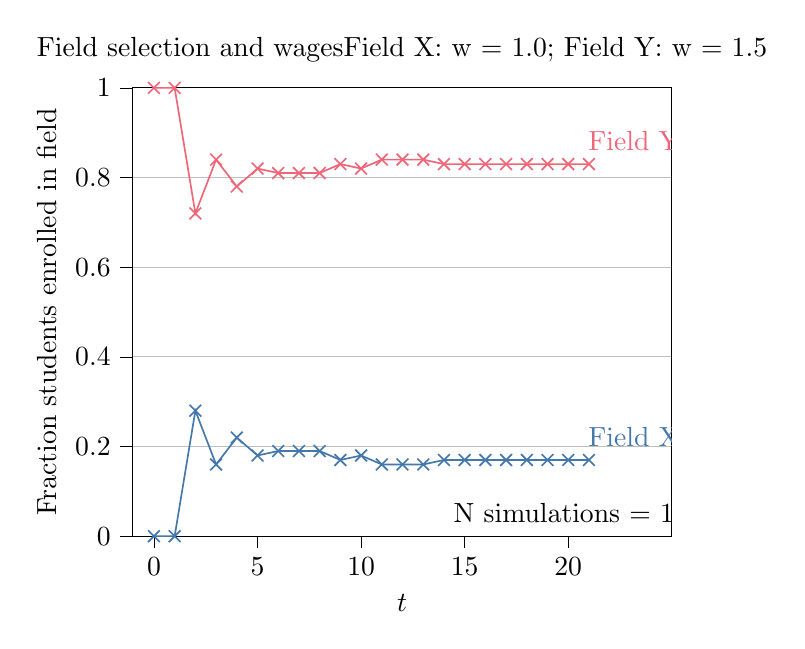
\begin{tikzpicture}

\definecolor{color0}{rgb}{0.266666666666667,0.466666666666667,0.666666666666667}
\definecolor{color1}{rgb}{0.933333333333333,0.4,0.466666666666667}

\begin{axis}[
height=207pt,
tick align=outside,
tick pos=left,
title={Field selection and wages \\ Field X: w = 1.0; Field Y: w = 1.5},
width=240pt,
x grid style={white!69.0196078431373!black},
xlabel={\(\displaystyle t\)},
xmin=-1.05, xmax=25,
xtick style={color=black},
xtick={0,5,10,15,20},
xticklabels={\(\displaystyle 0\),\(\displaystyle 5\),\(\displaystyle 10\),\(\displaystyle 15\),\(\displaystyle 20\)},
ylabel={Fraction students enrolled in field},
ymajorgrids,
ymin=0, ymax=1,
ytick style={color=black},
ytick={0,0.2,0.4,0.6,0.8,1},
yticklabels={\(\displaystyle 0\),\(\displaystyle 0.2\),\(\displaystyle 0.4\),\(\displaystyle 0.6\),\(\displaystyle 0.8\),\(\displaystyle 1\)}
]
\addplot [semithick, color0, mark=x, mark size=3, mark options={solid}]
table {%
0 0
1 0
2 0.28
3 0.16
4 0.22
5 0.18
6 0.19
7 0.19
8 0.19
9 0.17
10 0.18
11 0.16
12 0.16
13 0.16
14 0.17
15 0.17
16 0.17
17 0.17
18 0.17
19 0.17
20 0.17
21 0.17
};
\addplot [semithick, color1, mark=x, mark size=3, mark options={solid}]
table {%
0 1
1 1
2 0.72
3 0.84
4 0.78
5 0.82
6 0.81
7 0.81
8 0.81
9 0.83
10 0.82
11 0.84
12 0.84
13 0.84
14 0.83
15 0.83
16 0.83
17 0.83
18 0.83
19 0.83
20 0.83
21 0.83
};
\draw (axis cs:20.5,0.2) node[
  anchor=base west,
  text=color0,
  rotate=0.0
]{Field X};
\draw (axis cs:20.5,0.86) node[
  anchor=base west,
  text=color1,
  rotate=0.0
]{Field Y};
\draw (axis cs:14,0.03) node[
  anchor=base west,
  text=black,
  rotate=0.0
]{N simulations = 100};
\end{axis}

\end{tikzpicture}
